\newcommand{\arrowWidth}{1.7pt}
\newcommand{\rectWidth}{0.5cm}
\newcommand{\circleSize}{0.9cm}
\begin{figure*}[htp]
%
\begin{center}
\begin{subfigure}[t]{0.45\textwidth}
\begin{tikzpicture}
\path (0.0,0.0) node[rectangle,draw,minimum size=\circleSize,align=center](x) {
    $x$ 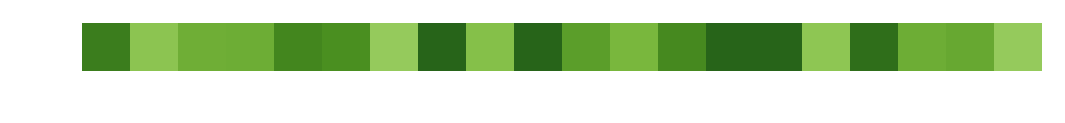
\includegraphics[scale=0.25]{x.eps}\\\small non-sensitive observations
}
(4.2,0.0) node[rectangle,draw,minimum size=\circleSize,align=center](a) {
    $a$ 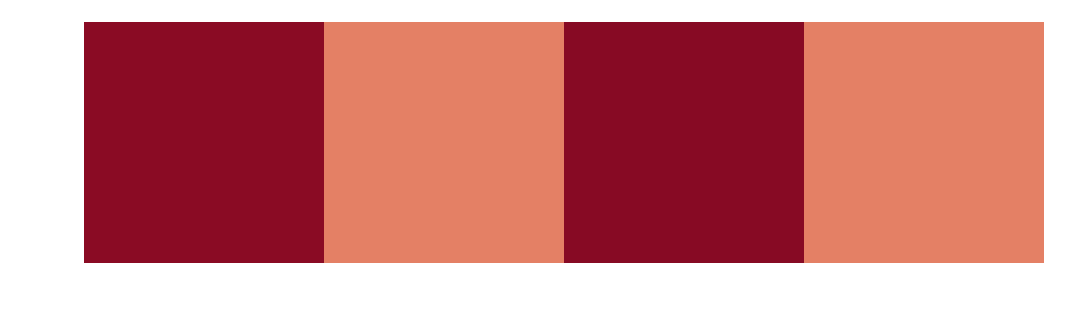
\includegraphics[scale=0.08]{a.eps}\\\small sensitive observations
}
(0.0,3.0) node[rectangle,draw,minimum size=\circleSize,align=center](z) {
    $z$ 
\includegraphics[scale=0.2]{z.eps}\\\small non-sensitive latents
}
(4.2,3.0) node[rectangle,draw,minimum size=\circleSize,align=center](b) {
    $b$ 
\includegraphics[scale=0.08]{b.eps}\\\small sensitive latents
};
\draw[->,>=stealth, line width=\arrowWidth] (x) to [out=45,in=-45,looseness=1.0] (z);
\draw[->,>=stealth, line width=\arrowWidth] (z) to [out=-135,in=135,looseness=1.0] (x);
\draw[->,>=stealth, line width=\arrowWidth] (x) to [out=20,in=-110,looseness=1.0] (b);
\draw[->,>=stealth, line width=\arrowWidth] (b) to [out=-130,in=40,looseness=1.0] (x);
\draw[->,>=stealth, line width=\arrowWidth] (b) -- (a);
\end{tikzpicture}
    \caption{
    FFVAE learns the encoder distribution $q(z,b|x)$ and decoder distributions $p(x|z,b)$, $p(a|b)$ from inputs $x$ and multiple sensitive attributes $a$.
    The disentanglement prior structures the latent space by encouraging low $\text{MI}(b_i,a_j)\forall i \neq j$ and low $\text{MI}(b,z)$ where $\text{MI}(\cdot)$ denotes mutual information.
    }
\label{fig:1a}
\end{subfigure}
%
\hfill
%
\begin{subfigure}[t]{0.45\textwidth}
\begin{tikzpicture}
\path
(0.0-1.8,0.0) node[rectangle,draw,minimum size=\circleSize,align=center](x) {
    $x$ 
\includegraphics[scale=0.25]{x_test.eps}
}
(0.0-1.8,2.2) node[rectangle,draw,minimum size=\circleSize,align=center](z) {
    $z$ 
\includegraphics[scale=0.2]{z_test.eps}
}
(4.0-1.8,1.1) node[rectangle,draw,minimum size=\circleSize,align=center](b) {
    $b$ 
\includegraphics[scale=0.08]{b_test.eps}
}
(4.0-1.8,2.5) node[rectangle,draw,minimum size=\circleSize,align=center](bprime) {
    $b'$ 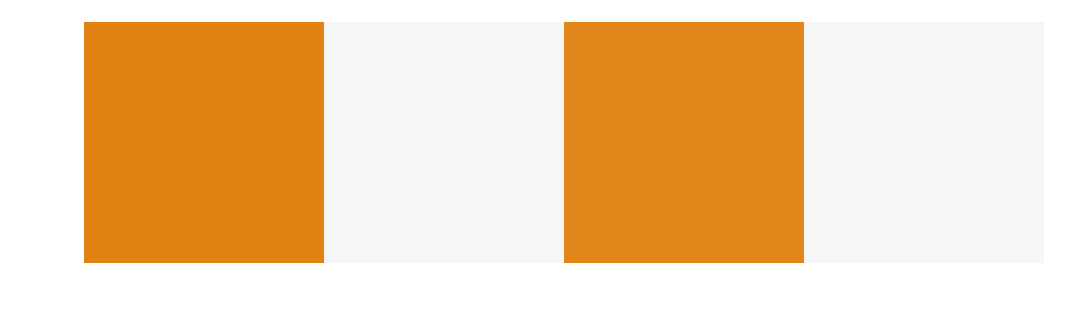
\includegraphics[scale=0.08]{b_after_test.eps}\\\scriptsize modified sens. latents
}
(2.0-1.8,4.0) node[rectangle,draw,minimum size=\circleSize,align=center](y) {
    $y$ 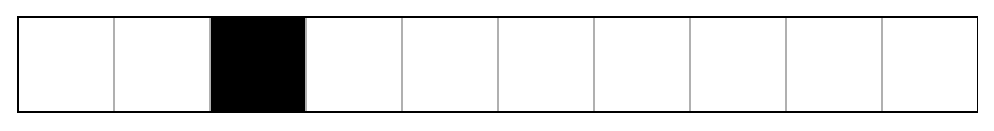
\includegraphics[scale=0.2]{y.eps}\\\small target label
};
\draw[->,>=stealth, line width=\arrowWidth] (x) -- (z);
\draw[->,>=stealth, line width=\arrowWidth] (x) to [out=0,in=-90,looseness=1.6] (b);
\draw[->,>=stealth, line width=\arrowWidth] (b) -- (bprime);
\draw[->,>=stealth, line width=\arrowWidth] (bprime) -- (y);
\draw[->,>=stealth, line width=\arrowWidth] (z) -- (y);
\end{tikzpicture}
    \caption{The FFVAE latent code $[z,b]$ can be modified by discarding or noising out sensitive dimensions $\{b_j\}$, which yields a latent code $[z, b']$ independent of groups and subgroups derived from sensitive attributes $\{a_j\}$.
A held out label $y$ can then be predicted with subgroup demographic parity.
}

\label{fig:1b}
\end{subfigure}
\caption{
    Data flow at train time (\ref{fig:1a}) and test time (\ref{fig:1b}) for our model, Flexibly Fair VAE (FFVAE).
}
\label{modelpic}
\end{center}
\vskip -0.2in
\label{fig:1}
\end{figure*}

